\section{How to Find the Best Policy?}

\begin{frame}
    \frametitle{Table of contents}
    \tableofcontents
\end{frame} 



\begin{frame}
    \frametitle{How to Find the Best Policy?}
    Methods:
    \begin{itemize}
        \item Dynamic Programming:
        \begin{itemize}
            \item Policy Iteration;
            \item Value Iteration;
        \end{itemize}
        \item RL Algorithms:
        \begin{itemize}
            \item TD-learning.
            \item Q-learning;
            %\item Sarsa;
        \end{itemize}
    \end{itemize}
\end{frame} 

\subsection{Dynamic Programming}
\begin{frame}
    \frametitle{Dynamic Programming}

    \begin{itemize}
        \item Dynamic Programming (DP) is a very general solution method for
        problems which have two properties:

        \begin{itemize}
            \item Optimal solution can be decomposed into subproblems;
            \item Subproblems recur many times (solutions can be cached and reused);
        \end{itemize}

        \item Markov decision processes (MDP) satisfy both properties:
        \begin{itemize}
            \item Bellman equation gives recursive decomposition;
            \item Value function stores and reuses solutions.
        \end{itemize}

        \item {\color{red}Model based-approch:} Dynamic Programming assumes full 
        knowledge of the MRP environment ($\mathcal{P}_{ss'}^{a}$ and $\mathcal{R}_{s}^{a}$)
    \end{itemize}
\end{frame} 




\subsubsection{Policy Iteration}

\begin{frame}
    \frametitle{Policy Iteration}

    Algorithm steps:
    \begin{itemize}
        \item Policy evaluation;
        \item Policy improvement.
    \end{itemize}

\end{frame} 



\begin{frame}
    \frametitle{Policy Iteration (Evaluation)}
    %\begin{block}{Policy Improvement}
        \begin{algorithmic}[]
            %\INPUT $\theta$: a small number
            \STATE Given the policy $\pi(s)$
            \STATE Initialize $V(s) = 0~\forall s\in\mathcal{S}$
            \break
            \WHILE{$\Delta < \Theta$ (a small threshold)}
                \FOR{each $s \in \mathcal{S}$}
                    $v \leftarrow V(s)$
                    $V(s) \leftarrow\sum_{a\in\mathcal{A(s)}}\pi(s|a)\sum_{s'\in\mathcal{S}}p(s'|s,a)[R(s)+\gamma~V(s')]$
                    $\Delta\leftarrow max(\Delta, |v-V(s)|)$
                \ENDFOR{}
            \ENDWHILE{}      
            \break
            \RETURN $V$: a value function

        \end{algorithmic}
    %\end{block}

\end{frame} 



\begin{frame}
    \frametitle{Policy Iteration (Grid World Example)}
    Evaluation step:
    \begin{figure}
        \centering
        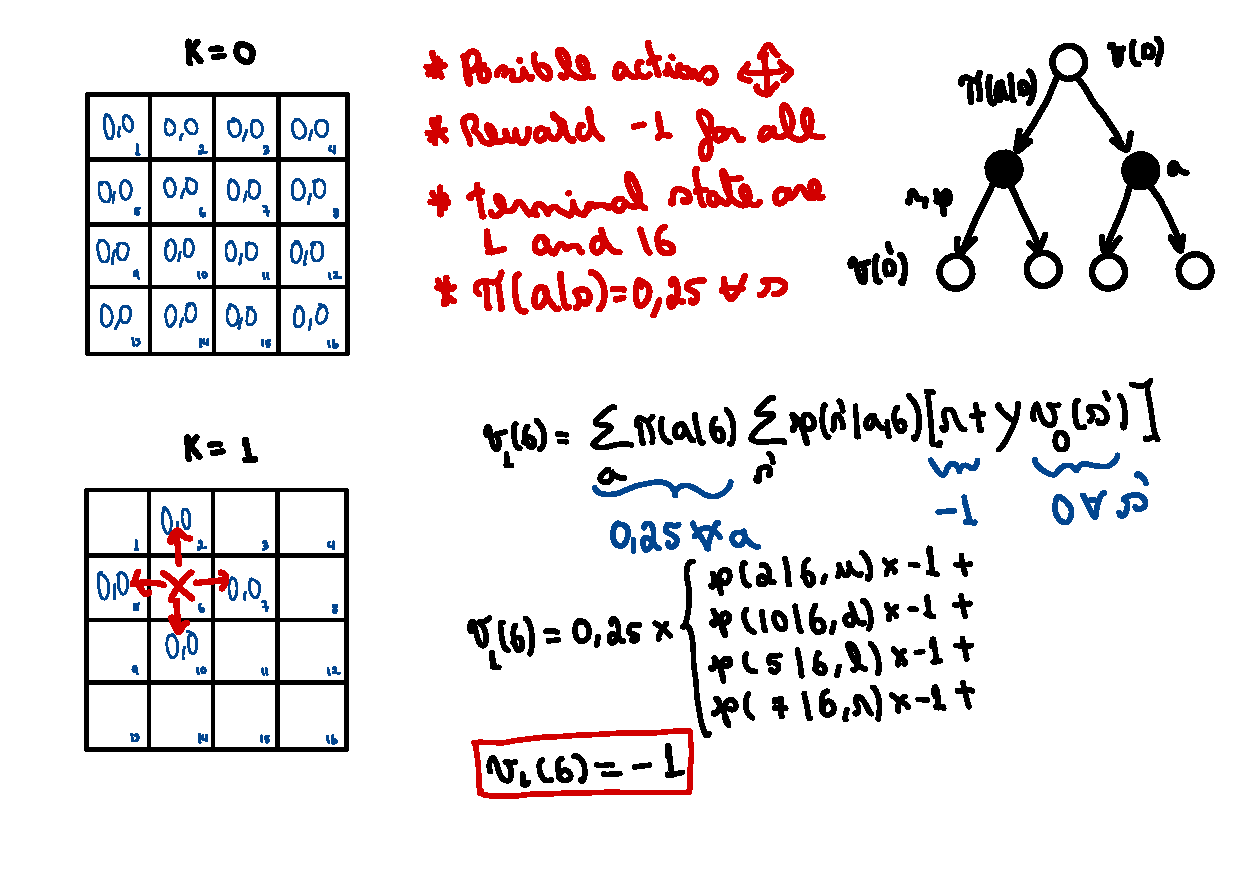
\includegraphics[width=0.9\textwidth]{sections/optimization/figures/grid_world_pi_1.pdf}
    \end{figure}
\end{frame}

\begin{frame}
    \frametitle{Policy Iteration (Grid World Example)}
    Evaluation step:

    \begin{figure}
        \centering
        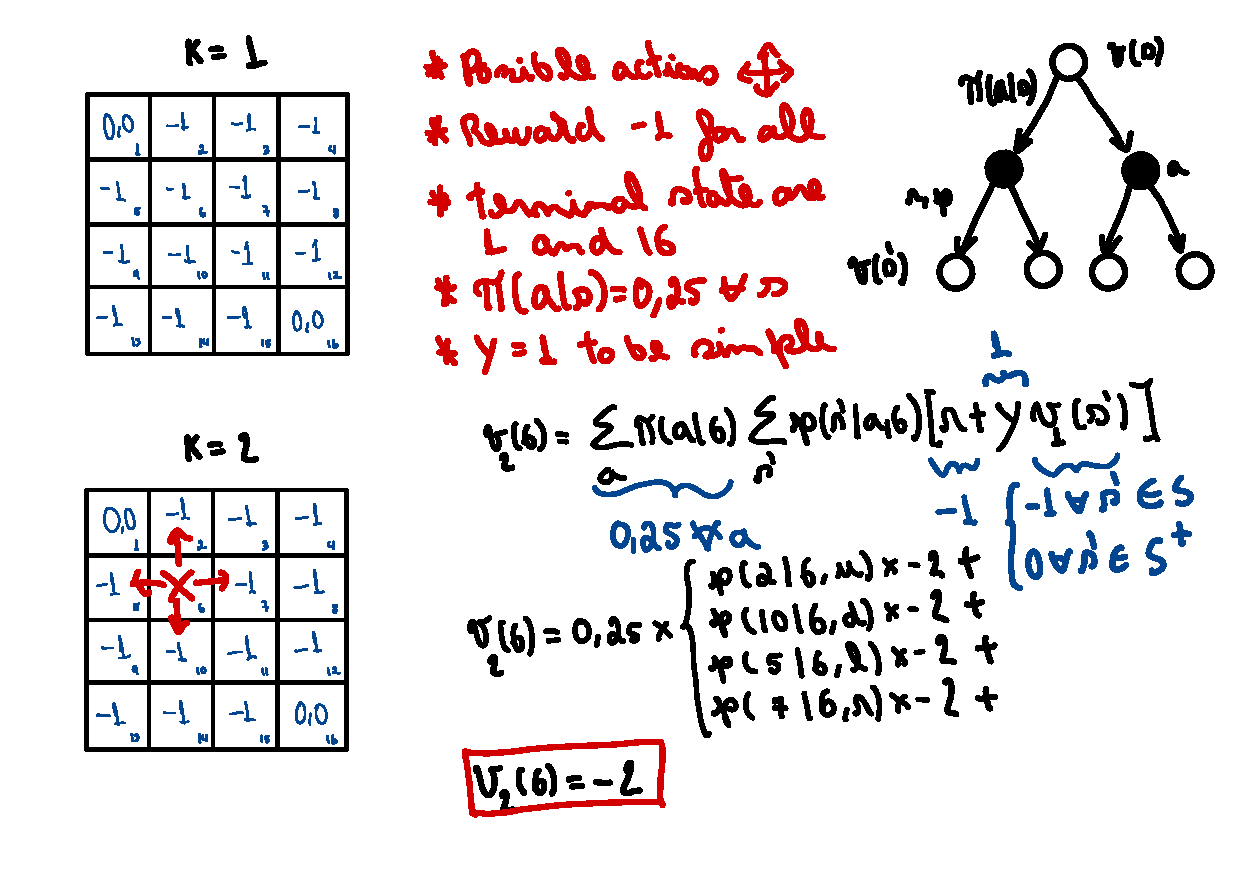
\includegraphics[width=0.9\textwidth]{sections/optimization/figures/grid_world_pi_2.pdf}
    \end{figure}
\end{frame}





\begin{frame}
    \frametitle{Policy Iteration (Grid World Example)}
    Evaluation step: $\Delta$ convergence.
    \begin{figure}
        \centering
        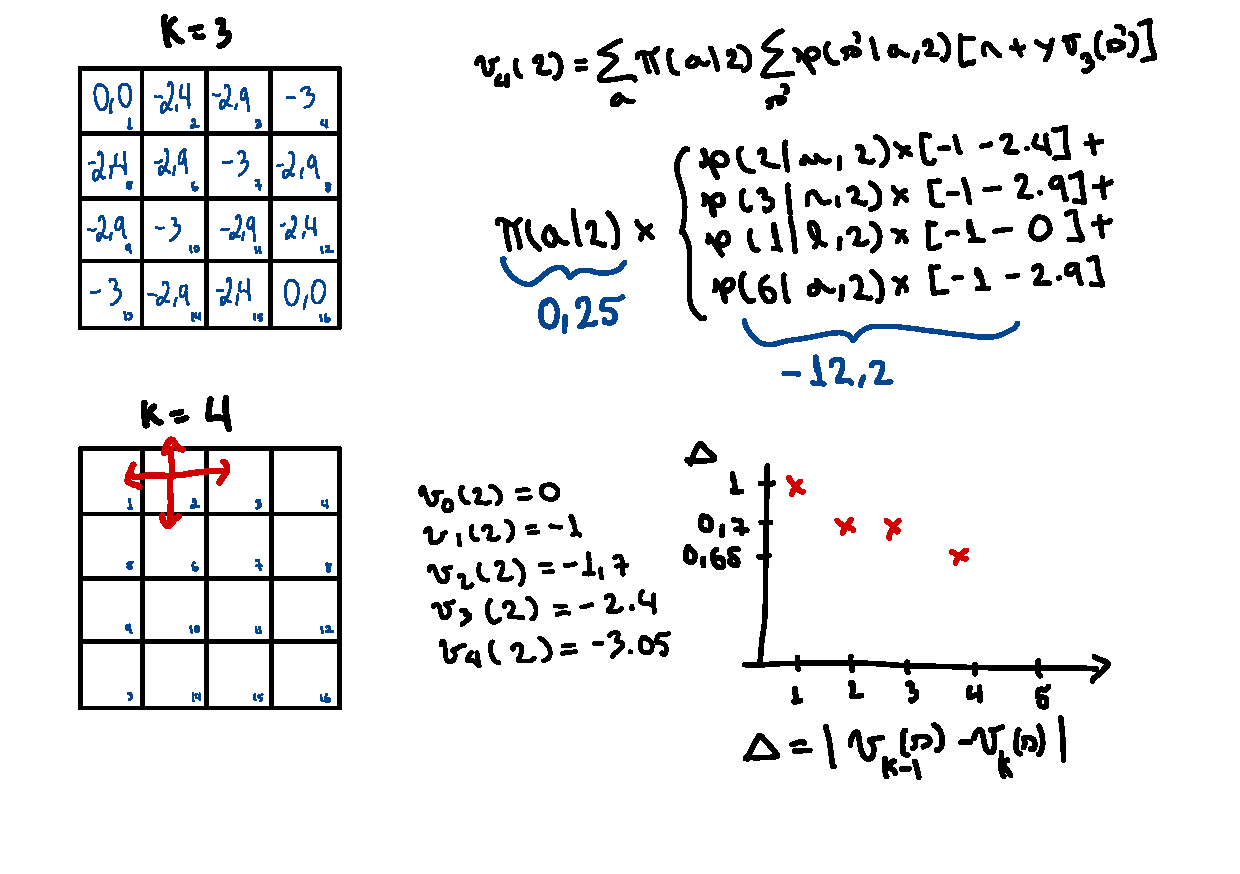
\includegraphics[width=0.9\textwidth]{sections/optimization/figures/grid_world_pi_3.pdf}
    \end{figure}
\end{frame}

\begin{frame}
    \frametitle{Policy Iteration (Grid World Example)}
    Evaluation step:
    \begin{figure}
        \centering
        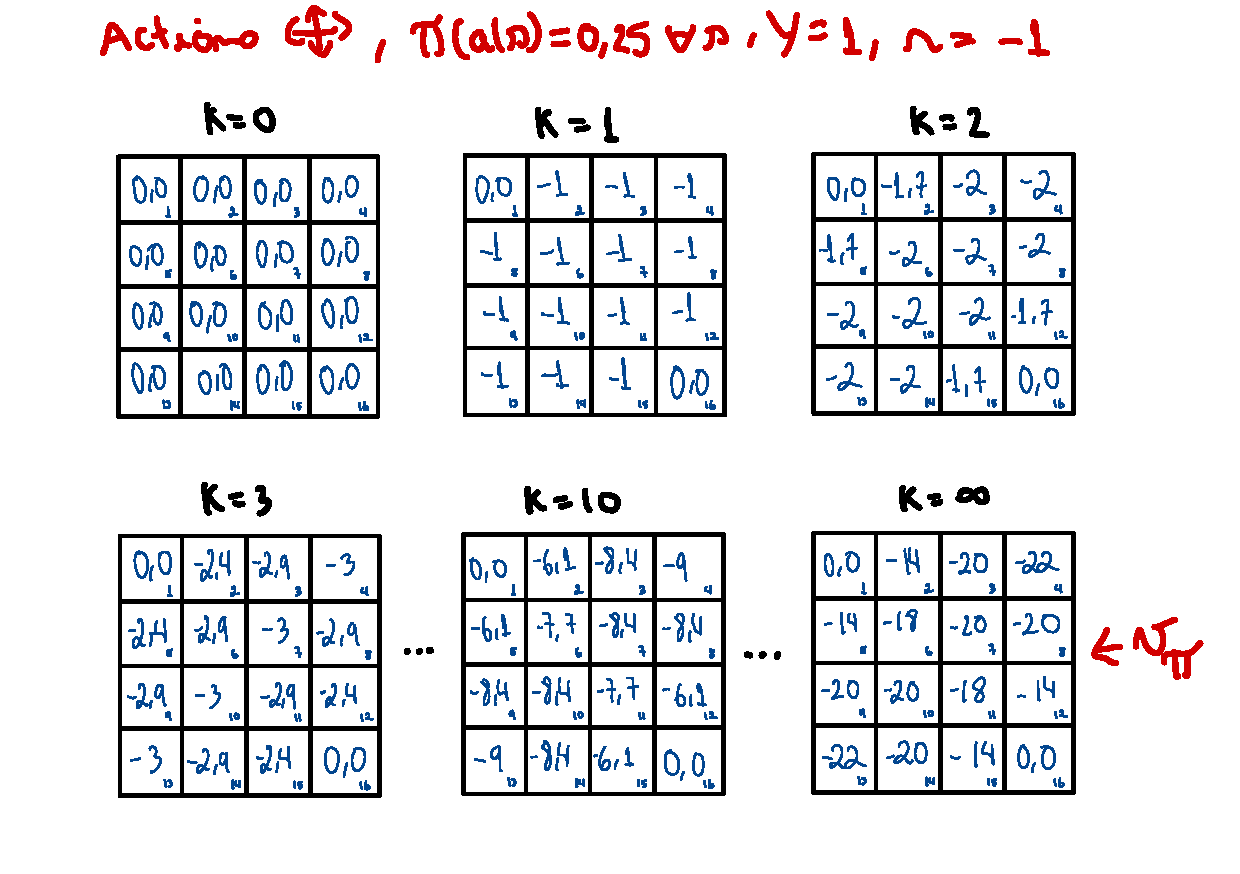
\includegraphics[width=0.9\textwidth]{sections/optimization/figures/grid_world_pi_4.pdf}
    \end{figure}
\end{frame}

\begin{frame}
    \frametitle{Policy Iteration (Improvement)}
    %\begin{block}{Policy Improvement}
        \begin{algorithmic}[1]
            %\INPUT $\theta$: a small number
            \STATE Initialize $\pi~\forall s \in \mathcal{S}$, to a random action $a \in \mathcal{A}(s)$, arbitrarily
            \break
            
            \REPEAT{}
                \STATE Compute $V$ for all states using a policy evaluation algorithm and the current policy $\pi(s)$\\
                
                \FOR{each $s \in \mathcal{S}$}
                    \STATE$\pi(s)\leftarrow argmax_{a}(\sum_{s'\in\mathcal{S}}p(s'|s,a)[R(s)+\gamma~V(s')])$
                \ENDFOR{}
            \UNTIL{$\pi(s) = \pi'(s)~\forall~s$}    
            \break
            \RETURN $\pi$: policy function

        \end{algorithmic}
    %\end{block}

\end{frame} 




\begin{frame}
    \frametitle{Policy Iteration (Grid World Example)}
    Optimization step:
    \begin{figure}
        \centering
        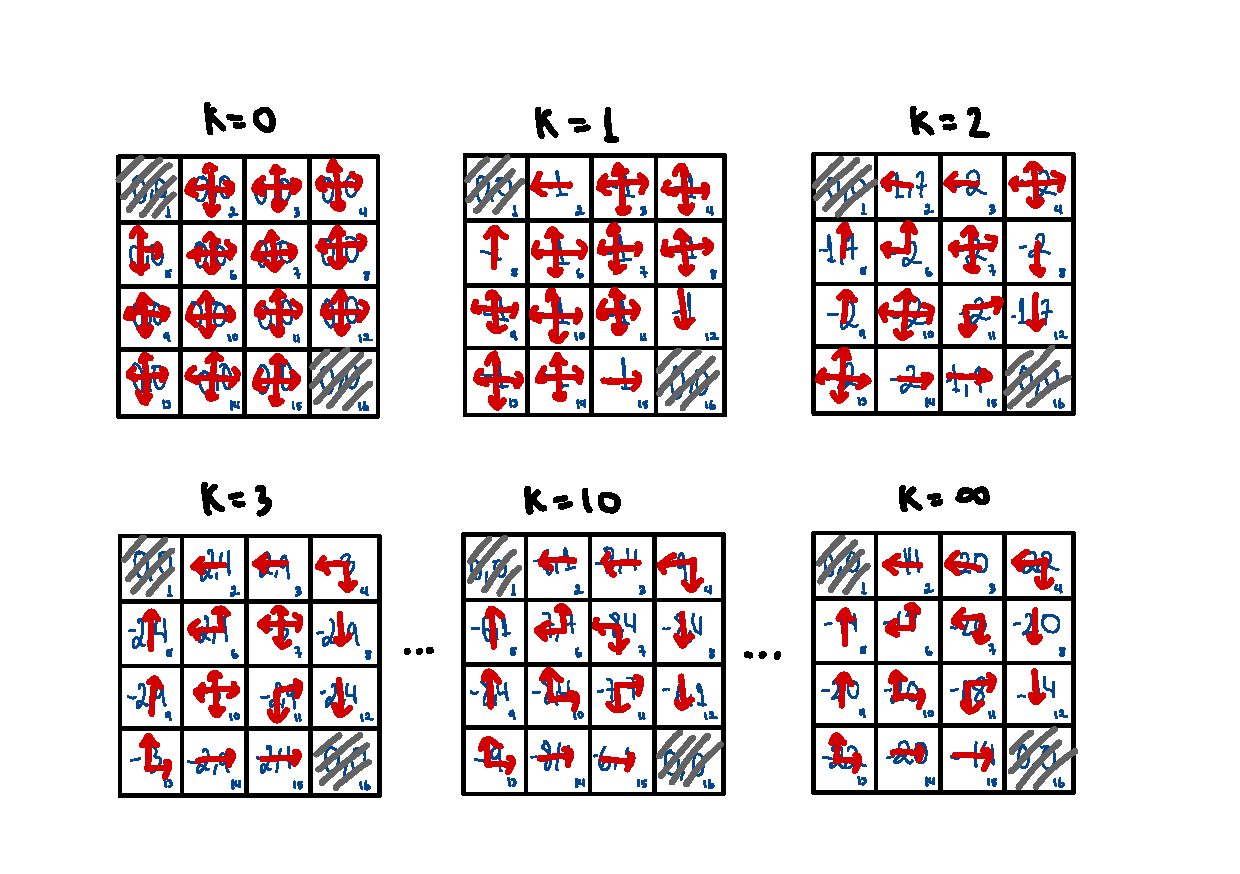
\includegraphics[width=0.9\textwidth]{sections/optimization/figures/grid_world_pi_5.pdf}
    \end{figure}
\end{frame}


\subsubsection{Value Iteration}

\begin{frame}
    \frametitle{Value Iteration}

    In value interation, we compute the optimal state value function 
    by iteratively updating the estimate $V(s)$.
    %\begin{block}{Policy Improvement}
        \begin{algorithmic}[1]
            %\INPUT $\theta$: a small number
            \STATE Initialize $\pi~\forall s \in \mathcal{S}$, to a random action $a \in \mathcal{A}(s)$, 
            $V(s)$ arbitrarily and $V(terminal)\leftarrow~0$  
        
            \WHILE{$\Delta < \Theta$ (a small threshold)}
                \FOR{each $s \in \mathcal{S}$}
                    $v \leftarrow V(s)$
                    $V(s) \leftarrow max_{a}\sum_{s'\in\mathcal{S}}p(s'|s,a)[R(s)+\gamma~V(s')]$
                    $\Delta\leftarrow max(\Delta, |v-V(s)|)$
                \ENDFOR{}
            \ENDWHILE{}        
            \break
            $\pi_{*}(s) = argmax_{a}\sum_{s'\in\mathcal{S}}p(s'|s,a)[R(s)+\gamma~V(s')]~\forall~s~\in~\mathcal{S}$ 
            \RETURN $\pi_{*}$
        \end{algorithmic}
    %\end{block}

\end{frame} 

\begin{frame}
    \frametitle{Value Iteration (Grid World Example)}
    \begin{figure}
        \centering
        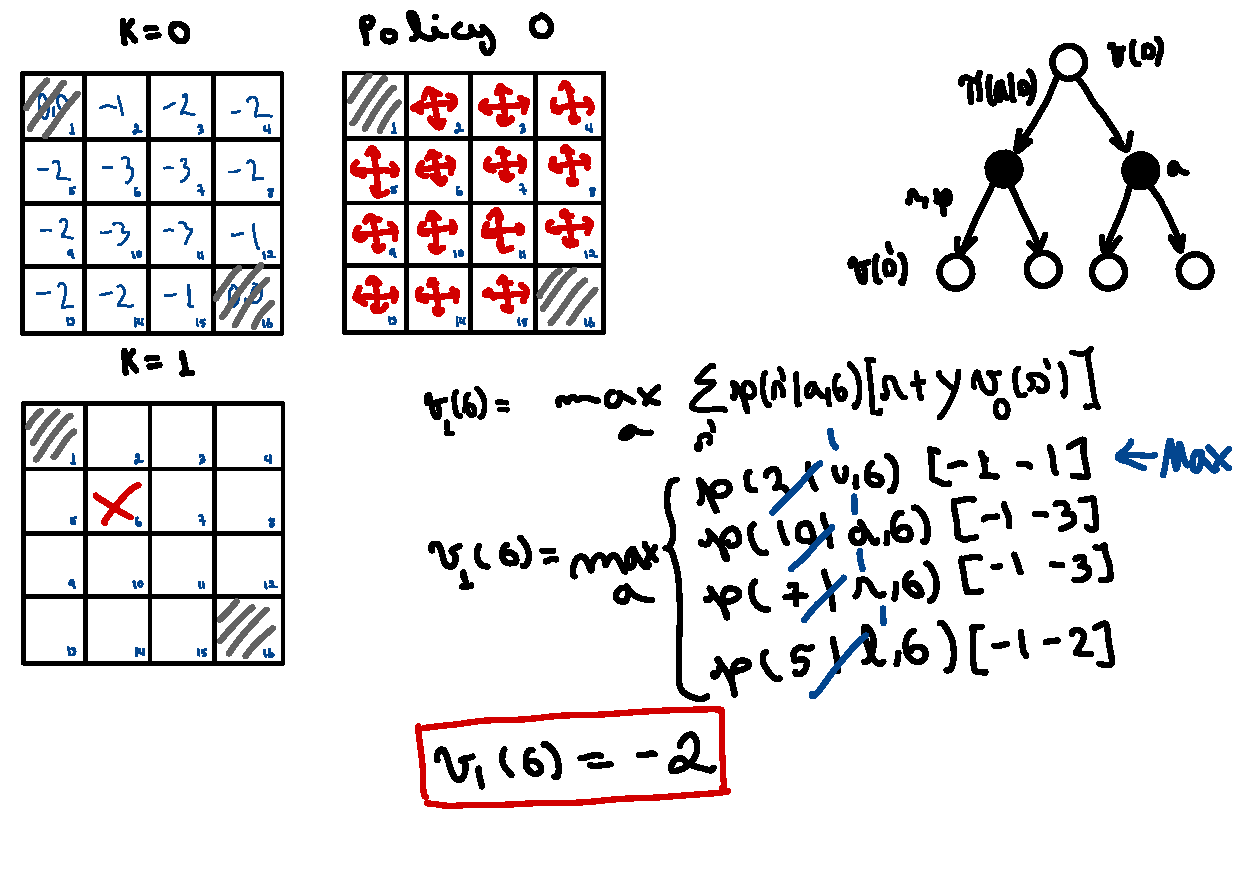
\includegraphics[width=0.9\textwidth]{sections/optimization/figures/grid_world_vi_1.pdf}
    \end{figure}
\end{frame}



\begin{frame}
    \frametitle{Policy or Value Iteration?}
    \begin{itemize}
        \item Number of iteration in policy iteration before convergence is polynomial, and usually needs 
        less iterations to stop than Value iteration;
        \item Value iteration needs a lot of iterations to converge to small errors, however, value iteration 
        converges to optimal policy long before it converges to correct value in this MDP;
        \item Policy iteration requires fewer iterations that value iteration, but each iteration requires 
        solving a linear system instead of just applying Bellman operator;
        \item In practice, policy iteration is often faster, especially if the transition probabilities 
        are structured (e.g., sparse) to make solution of linear system efficient.
    \end{itemize}
\end{frame}



\begin{frame}
    \frametitle{How to Find the Best Policy?}
    Methods:
    \begin{itemize}
        \item Dynamic Programming:
        \begin{itemize}
            \item Policy Iteration;
            \item Value Iteration;
        \end{itemize}
        
        \item {\color{red}RL Algorithms:}
        \begin{itemize}
            \item TD-learning.
            \item Q-learning;
            %\item Sarsa;
        \end{itemize}
        
    \end{itemize}
\end{frame} 


\subsection{RL Algorithms}


\subsubsection{TD-learning}
\subsubsection{Q-learning}


\begin{frame}
    \frametitle{Q-learning}
    \begin{itemize}
        \item Is a {\color{red}model-free} RL algorithm;
        \item Uses Q-values (also called action values) to iteratively improve 
        the behavior of the learning agent;
        \item  This estimation of $Q(S,A)$ will be iteratively computed 
        using the TD-Update rule;
        \item The Temporal Difference or TD-Update rule can be represented 
        as follows:
        $$q_{k+1}(s,a) = q_{k}(s,a) + \alpha[r+\gamma~q_{k}(s',a') - q_{k}(s,a)]$$
        \item Since we don't know anything about the environment, let's use exploration and 
        exploitation strategy.
    \end{itemize}
\end{frame}

\begin{frame}
    \frametitle{Q-learning Algorithm (Example)}
    \begin{figure}
        \centering
        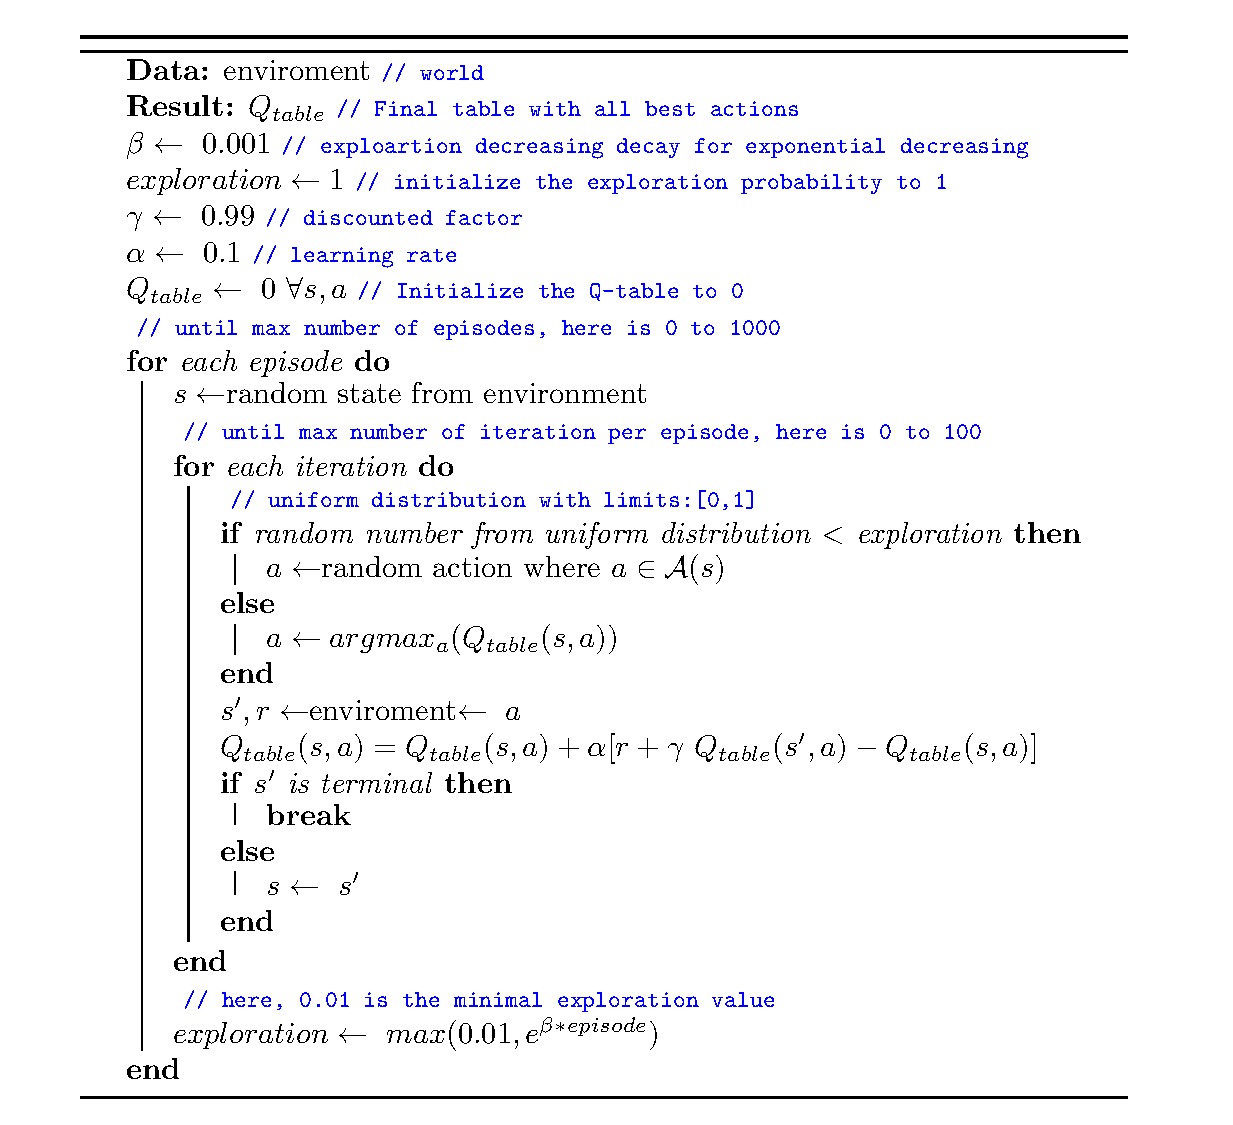
\includegraphics[width=0.7\textwidth]{sections/optimization/figures/q_learning_alg.pdf}
    \end{figure}
\end{frame}



